\documentclass{article}

% Language setting
% Replace `english' with e.g. `spanish' to change the document language
\usepackage[english]{babel}

% Set page size and margins
% Replace `letterpaper' with `a4paper' for UK/EU standard size
\usepackage[letterpaper,top=2cm,bottom=2cm,left=3cm,right=3cm,marginparwidth=1.75cm]{geometry}

% Useful packages
\usepackage{amsmath}
\usepackage{minted}
\usepackage{graphicx}
\usepackage{listings}
\usepackage[utf8]{inputenc}
\usepackage[hidelinks]{hyperref}
\usepackage{geometry}
\usepackage[colorlinks=true, allcolors=blue]{hyperref}











\title{QEMU NXP  S32K3X8EVB   Board Documentation}
\author{Andrea Mugnaini, Giovanni Amendolia, Giuseppe Maganuco}

\begin{document}
\maketitle


\section{Introduction}

The S32K3X8EVB-Q289 is an evaluation and development board for general-purpose automotive and industrial applications.

Based on the 32-bit Arm\textsuperscript{\textregistered}Cortex\textsuperscript{\textregistered}-M7 S32K3 MCU in a 289 MAPBGA package, the S32K3X8EVB-Q289 offers a multicore mode, Hardware Security Engine (HSE), Over-the-Air (OTA) support, advanced connectivity and low power.

The S32K3X8EVB-Q289 offers a standard-based form factor compatible with the Arduino® pin layout, providing a broad range of expansion board options for quick application prototyping.\cite{nxp_s32k3xxrm}

\section{Getting Started}

\subsection{Repository Layout}
\begin{minted}[fontsize=\small, bgcolor=gray!5, frame=single]{text}
group9/
├── firmware/      # FreeRTOS firmware and board drivers
│   ├── FreeRTOSConfig.h
│   ├── Makefile
│   ├── adc.c / adc.h
│   ├── uart.c / uart.h
│   ├── linker.ld
│   ├── startup.c
│   ├── main.c
│   └── qemu-debug-log   #Qemu UART and ADC Log for debugging
├── qemu/          # Custom QEMU source for nxps32k3x8evb
└── documentation/          # Documentation and guides
\end{minted}

\subsection{Build QEMU}
The steps followed the paper \textbf{"Tame the QEMU", SSTIC 2024
} \cite{sstic‐tame‐the‐qemu} for implementing a custom board with pluggable peripherals.
\subsubsection{Register Files in Meson Build System}


QEMU uses \texttt{meson.build} to manage sources, update the build file with the correct sources for the board and the Memory Control Unit.


\begin{minted}[fontsize=\small, bgcolor=gray!5, frame=single]{text}
# qemu/hw/arm/meson.build
arm_ss.add(when: 'CONFIG_S32K3X8EVB', if_true: files(
  's32k3x8evb.c',
  's32k3x8evb_mcu.c',
))
\end{minted}
\newline
\newpage
\textbf{UART:}
\begin{minted}[fontsize=\small, bgcolor=gray!5, frame=single]{text}
# qemu/hw/char/meson.build
softmmu_ss.add(when: 'CONFIG_S32K3X8EVB', if_true: files(
  'nxps32k3x8evb_uart.c',
))
\end{minted}

\textbf{ADC:}


\begin{minted}[fontsize=\small, bgcolor=gray!5, frame=single]{text}
# qemu/hw/adc/meson.build
softmmu_ss.add(when: 'CONFIG_S32K3X8EVB', if_true: files(
  'nxps32k3x8evb_adc.c',
))
\end{minted}



\subsubsection{Add Kconfig Entry}

Enable your board in \texttt{qemu/hw/arm/Kconfig}:
\begin{minted}[fontsize=\small, bgcolor=gray!5, frame=single]{text}
config S32K3X8EVB
    bool
    default y

\end{minted}


\subsubsection{Rebuild QEMU with the New Board}

Once all files and configs are added:
\begin{minted}[fontsize=\small, bgcolor=gray!5, frame=single]{bash}
# From QEMU root directory
mkdir build && cd build
../configure --target-list=arm-softmmu
make -j$(nproc)
\end{minted}

After compilation, your board appears as:
\begin{minted}[fontsize=\small, bgcolor=gray!5, frame=single]{bash}
#From the build directory
./qemu-system-arm -machine help | grep s32k3x8evb
\end{minted}



\subsection{Build the Firmware}
\subsubsection*{Requirements}
\begin{minted}[fontsize=\small, bgcolor=gray!5, frame=single]{bash}
sudo apt update
sudo apt install gcc-arm-none-eabi gdb-multiarch -y
\end{minted}


\subsubsection*{Available Make Commands}

\paragraph{Build the firmware}
Compiles all FreeRTOS and project sources, links them into a final ELF, and prints memory usage:
\begin{minted}[fontsize=\small, bgcolor=gray!5, frame=single]{bash}
make -j
\end{minted}

The \texttt{-j} flag enables parallel compilation for faster builds.

\paragraph{Install required dependencies}
Installation of the necessary dependencies for the project
\begin{minted}[fontsize=\small, bgcolor=gray!5, frame=single]{bash}
make init
\end{minted}

\paragraph{Clean the build}
Removes all build outputs, including ELF, MAP, and object files, so you can start fresh:
\begin{minted}[fontsize=\small, bgcolor=gray!5, frame=single]{bash}
make clean
\end{minted}

---

\paragraph{Run in QEMU}
After compiling, run the firmware on the custom QEMU machine:
\begin{minted}[fontsize=\small, bgcolor=gray!5, frame=single]{bash}
make qemu_start
\end{minted}

This internally launches:
\begin{minted}[fontsize=\small, bgcolor=gray!5, frame=single]{bash}
../../qemu/build/qemu-system-arm \
    -machine nxps32k3x8evb \
    -kernel Output/firmware.elf \
    -nographic -D ./qemu-debug-log
\end{minted}

\begin{itemize}
  \item \textbf{-machine}: Custom board model for QEMU.
  \item \textbf{-kernel}: Loads the compiled ELF directly into memory.
  \item \textbf{-nographic}: Runs without GUI (UART logs only).
  \item \textbf{-D}: Saves QEMU logs to \texttt{qemu-debug-log}.
\end{itemize}

---

\paragraph{Debugging}
Enable debugging by adding \texttt{-s -S} to the \texttt{QEMU\_FLAGS} variable in the Makefile.  
Then:
\begin{enumerate}
  \item Terminal 1 — Start QEMU and wait for GDB:
  \begin{minted}[fontsize=\small, bgcolor=gray!5, frame=single]{bash}
make qemu_debug
  \end{minted}

  \item Terminal 2 — Connect with GDB:
  \begin{minted}[fontsize=\small, bgcolor=gray!5, frame=single]{bash}
arm-none-eabi-gdb Output/firmware.elf
(gdb) target remote :1234
(gdb) monitor reset halt
(gdb) load
(gdb) continue
  \end{minted}
\end{enumerate}



\section{Hardware Emulation}

\subsection{Memory Control Unit}
In real hardware, the MCU is tasked with mapping instructions/data from the physical memory in the CPU virtual address space.
In the QEMU QOM model, each type of physical memory in the device 
(ITCM, program flash, SRAM, data flash) is modeled as a separate 
\texttt{MemoryRegion} structure.

\begin{minted}[fontsize=\small, linenos, frame=single]{c}
struct NXPS32K3X8EVB_MCUState {
    SysBusDevice parent_obj;   // attach to system bus
    ARMv7MState cpu;           // Cortex-M core state

    MemoryRegion itcm;         // instruction tightly-coupled memory
    MemoryRegion pflash;       // program flash
    MemoryRegion sram;         // system RAM
    MemoryRegion dflash;       // data flash

    uint32_t itcm_size, pflash_size;
    uint32_t sram_size, dflash_size;
    MemoryRegion *board_memory;
    MemoryRegion container;    // parent container
    Clock *sysclk;             // system clock
};

\end{minted}
The MCU component is implemented using different steps, following QEMU DOM API standards:
\begin{itemize}
    \item \textbf{Initialization of the MCU instance.}
    \item \textbf{Memory region setup and mapping.}
    \item \textbf{System clock creation and connection.}
\end{itemize}

The initialization function sets up the CPU and the memory container:

\begin{minted}[fontsize=\small, frame=single, linenos]{c}
// Initialize container and Cortex-M7 CPU
NXPS32K3X8EVB_MCUState *s = NXPS32K3X8EVB_MCU(obj);
memory_region_init(&s->container, obj, "container", UINT64_MAX);
object_initialize_child(OBJECT(s), "armv7m", &s->cpu, TYPE_ARMV7M);
\end{minted}

Memory regions are created and mapped into the container. For example, ITCM:

\begin{minted}[fontsize=\small, frame=single, linenos]{c}
// Initialize ITCM memory blocks
for (int i = 0; i < ITCM_NUM; i++) {
    MemoryRegion *itcm_block = g_new0(MemoryRegion, 1);
    memory_region_init_ram(itcm_block, OBJECT(s), 
        g_strdup_printf("itcm%d", i), ITCM_BLOCK_SIZE, NULL);
    memory_region_add_subregion(&s->itcm, i*ITCM_BLOCK_SIZE, itcm_block);
}
memory_region_add_subregion(&s->container, ITCM_BASE_ADDRESS, &s->itcm);
\end{minted}

The system clock is created and connected to the CPU to emulate timing:

\begin{minted}[fontsize=\small, frame=single, linenos]{c}
// Create and connect system clock
s->sysclk = qdev_init_clock_in(DEVICE(s), "sysclk", NULL, NULL, 0);
clock_set_hz(s->sysclk, NXPS32K3X8_STD_CLK);
qdev_connect_clock_in(DEVICE(&s->cpu), "cpuclk", s->sysclk);
\end{minted}

Finally, the MCU type is registered in QEMU so that it can be displayed and selected:

\begin{minted}[fontsize=\small, frame=single, linenos]{c}
// Register MCU device type
static const TypeInfo nxps32k3x8evb_mcu_info = {
    .name = TYPE_NXPS32K3X8EVB_MCU,
    .parent = TYPE_SYS_BUS_DEVICE,
    .instance_size = sizeof(NXPS32K3X8EVB_MCUState),
    .instance_init = nxps32k3x8evb_mcu_init,
    .class_init = nxps32k3x8evb_mcu_class_init,
};
type_register_static(&nxps32k3x8evb_mcu_info);
\end{minted}
\newpage
\subsection{Memory Mapping}
The memory map of the NXP microcontroller is divided into 
\textbf{Flash Blocks} and \textbf{Peripheral Blocks}, each assigned 
fixed address ranges for program execution, data storage, and peripheral access.  

\paragraph{Flash Memory} \mbox{}\\
Flash blocks provide program storage, instruction memory, and data flash. 
The mapping is as follows:

\begin{figure}[H]
    \centering
    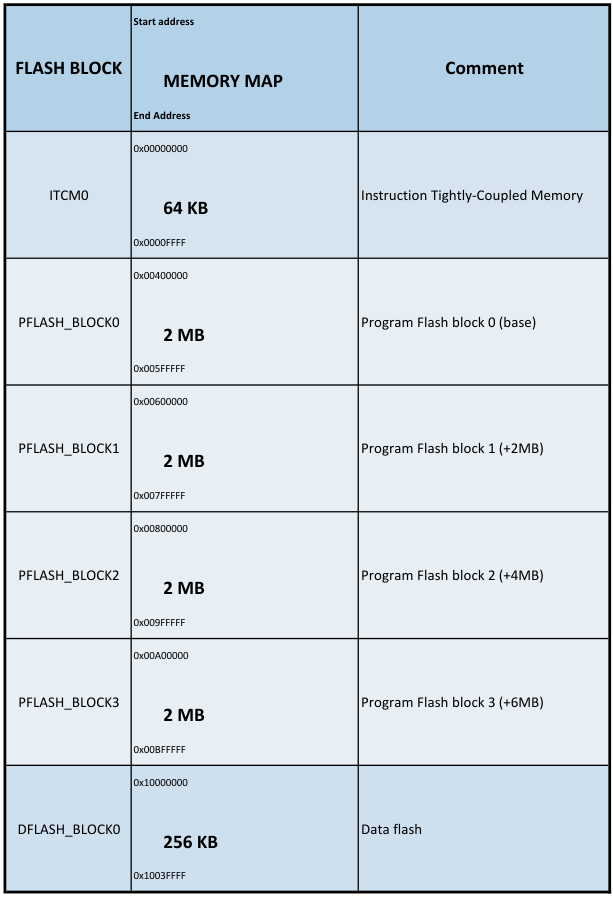
\includegraphics[width=0.85\textwidth]{images/memory_map_flash.png}
    \caption{Graphical representation of Flash memory mapping}
\end{figure}
\begin{figure}[H]
    \centering
    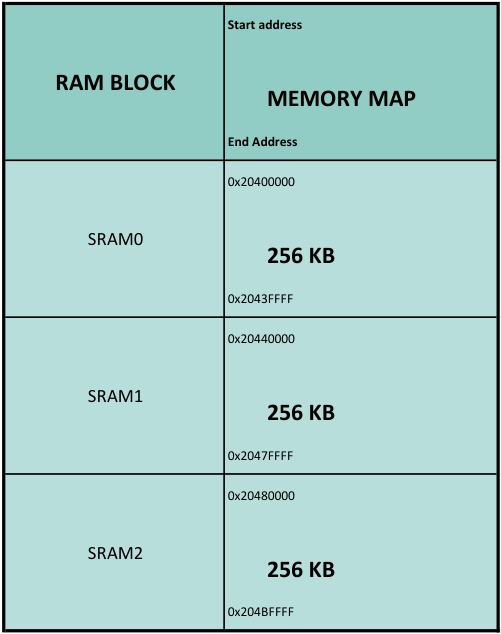
\includegraphics[width=0.85\textwidth]{images/Memory_map_flash.jpg}
    \caption{Graphical representation of SRAM memory mapping}
\end{figure}


\begin{itemize}
    \item \textbf{ITCM0}: It is a special memory, designed to store the instruction, that is directly connected to the CPU core, bypassing the cache. It is characterized by a deterministic time access. Used for critical code execution like Interrupt Service Routine (ISRs) 
    \textbf{[0x00400000 to 0x00BFFFFF]}
    \item \textbf{PFLASH\_BLOCK 0 to 3}: It is the non-volatile Flash memory where is stored the application code and constants.
    \textbf{[0x00000000 to 0x0000FFFF]}
    \item \textbf{DFLASH\_BLOCK0}: It is a region for non-volatile data storage. It founds usage for data that changes during runtime. It is typically smaller than the PFLASH (In fact 256 KB block size against 2 MB block size of the PFLASH). Typically it isn't used for code execution. \textbf{[0x10000000 to 0x1003FFFF]}

\end{itemize}

\paragraph{Peripheral Blocks}\mbox{}\\
Peripheral blocks are memory-mapped registers that control UART and ADC peripherals.

\begin{figure}[H]
    \centering
    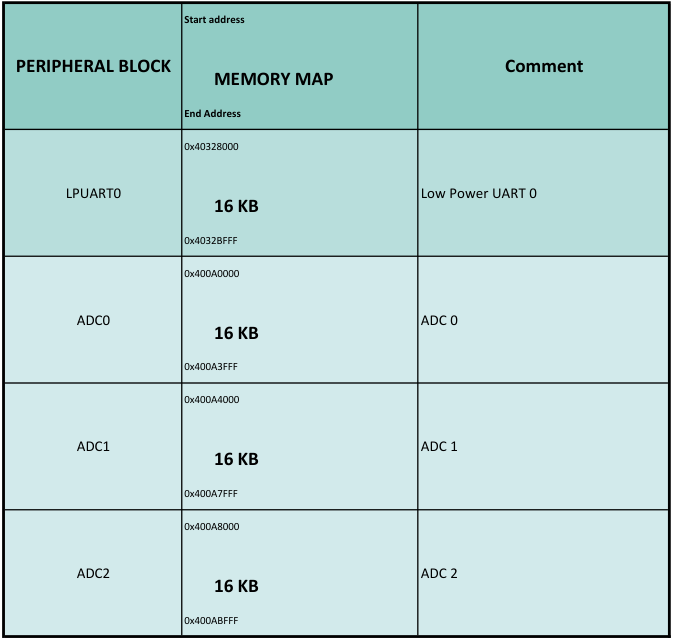
\includegraphics[width=0.85\textwidth]{images/memory_map_periph.png}
    \caption{Graphical representation of Peripheral memory mapping}
\end{figure}
\begin{itemize}
    \item \textbf{LPUART\_0}: A serial communication peripheral (UART) where 'LP' stands for Low Power.
    \textbf{[0x40328000 to 0x4032BFFF]}
    \item \textbf{ADC 0 to 2}: A module to convert analog voltages into digital values the CPU can process.
    \textbf{[0x400A0000 to 0x400ABFFF]}
\end{itemize}


\subsection{Board definition}



\subsection{UART}

The S32K3X8EVB board has multiple UART interfaces implemented through MCU’s
LPUART modules, enabling
serial communication with the PC for debugging. 
Another channel is brought out to the Arduino-compatible
headers, so that it can be connected to external devices.

The LPUART module supports standard asynchronous serial communication, with
programmable baud rates, parity, stop bits, and interrupt-driven operations, so that it makes it useful for tasks like debugging,
bootloader communication and external interfacing.

UART functionalities were modeled after the PrimeCell UART (PL011) module \cite{arm-pl011-0183G}, an Advanced Microcontroller Bus Architecture (AMBA) slave module that connects to the Advanced Peripheral Bus (APB) used for serial communications. It supports Direct Memory Access (DMA) operations, 32×8 transmit and 32×12 receive First-In, First-Out (FIFO) memory buffers.

This is the c structure modeling the UART device:
\begin{minted}[fontsize=\scriptsize, linenos, breaklines, frame=single]{c}
/* QEMU model of the ARM PrimeCell PL011 UART */
MemoryRegion iomem;              // Memory-mapped I/O region for UART registers
uint32_t flags;                  // Internal QEMU flags for configuration/state

uint32_t lcr;                    // Line Control Register (UARTLCR_H)
                                 // Controls word length, parity, stop bits, FIFO enable

uint32_t rsr;                    // Receive Status / Error Clear Register (UARTRSR/UARTECR)
                                 // Captures RX errors: framing, parity, break, overrun

uint32_t cr;                      // Control Register (UARTCR)
                                 // Enables TX/RX, UART, flow control signals

uint32_t dmacr;                   // DMA Control Register (UARTDMACR)
                                 // Controls DMA requests for RX/TX

uint32_t int_enabled;            // Interrupt Mask Set/Clear (UARTIMSC)
                                 // Which interrupts are enabled

uint32_t int_level;              // Interrupt status level
                                 // Mirrors UARTRIS/UARTMIS for raw/masked interrupt status

uint32_t read_fifo[NXP_UART_FIFO_DEPTH]; 
                                 // RX FIFO buffer (up to 32 entries)
                                 // Holds received data until read by CPU

uint32_t ilpr;                    // IrDA Low-Power Counter Register (UARTILPR)
                                 // Used for low-power infrared mode

uint32_t ibrd;                    // Integer Baud Rate Register (UARTIBRD)
                                 // Sets integer part of baud rate divisor

uint32_t fbrd;                    // Fractional Baud Rate Register (UARTFBRD)
                                 // Fine-tunes baud rate for precise clocking

uint32_t ifl;                      // Interrupt FIFO Level Select Register (UARTIFLS)
                                 // Sets RX/TX FIFO thresholds for interrupts

int read_pos;                      // Current read pointer index in RX FIFO
int read_count;                    // Current number of entries stored in RX FIFO
int read_trigger;                  // FIFO level threshold that triggers an RX interrupt

CharBackend chr;                  // QEMU character backend for host serial device connection

qemu_irq irq[6];                  // Emulated IRQ lines (RX, TX, timeout, modem, error, etc.)

Clock *clk;                        // Emulated UART reference clock

bool migrate_clk;                  // Migration flag for clock during VM save/restore

const unsigned char *id;          // Peripheral identification registers
\end{minted}

\newpage
The correlation between the hardware registers and the simulated ones is as follows:
\begin{table}[h!]
\centering
\caption{PL011 UART Register Mapping in \texttt{PL011State} Struct}
\begin{tabular}{|l|l|p{8cm}|}
\hline
\textbf{C Struct Field} & \textbf{Corresponding Register} & \textbf{Description} \\
\hline
\texttt{iomem} & Memory-mapped I/O & Represents the memory-mapped I/O region for the PL011 registers. \\
\hline
\texttt{flags} & -- & Internal status flags for UART operation (software only, not a hardware register). \\
\hline
\texttt{lcr} & \texttt{UARTLCR\_H} & Line Control Register: controls word length, parity, stop bits, and FIFO enable. \\
\hline
\texttt{rsr} & \texttt{UARTRSR/UARTECR} & Receive Status/Error Clear Register: overrun, parity, break, and framing error indicators. \\
\hline
\texttt{cr} & \texttt{UARTCR} & Control Register: enables/disables UART, TX/RX, flow control, and SIR mode. \\
\hline
\texttt{dmacr} & \texttt{UARTDMACR} & DMA Control Register: enables TX/RX DMA and controls DMA-on-error behavior. \\
\hline
\texttt{int\_enabled} & \texttt{UARTIMSC} & Interrupt Mask Set/Clear Register: masks/unmasks specific UART interrupts. \\
\hline
\texttt{int\_level} & \texttt{UARTIFLS} & Interrupt FIFO Level Select Register: defines TX/RX FIFO trigger levels for interrupts. \\
\hline
\texttt{read\_fifo[16]} & -- & Software FIFO buffer for received data, mirrors hardware FIFO when enabled. \\
\hline
\texttt{ilpr} & \texttt{UARTILPR} & IrDA Low-Power Counter Register: generates low-power IrDA pulses. \\
\hline
\texttt{ibrd} & \texttt{UARTIBRD} & Integer Baud Rate Register: integer part of baud rate divisor. \\
\hline
\texttt{fbrd} & \texttt{UARTFBRD} & Fractional Baud Rate Register: fractional part of baud rate divisor. \\
\hline
\texttt{ifl} & \texttt{UARTFR} & Flag Register: indicates TX/RX FIFO empty/full, UART busy, and modem input states. \\
\hline
\texttt{read\_pos} & -- & Tracks the current read position in the software FIFO. \\
\hline
\texttt{read\_count} & -- & Number of bytes currently in the software read FIFO. \\
\hline
\texttt{read\_trigger} & -- & Software FIFO level at which interrupts are triggered. \\
\hline
\texttt{chr} & -- & Character backend associated with the UART for I/O operations. \\
\hline
\texttt{irq[6]} & -- & Array of interrupt lines corresponding to the UART interrupts. \\
\hline
\texttt{clk} & -- & Pointer to the UART clock used for baud rate generation. \\
\hline
\texttt{migrate\_clk} & -- & Indicates whether the clock should migrate across VM snapshots. \\
\hline
\texttt{id} & \texttt{UARTPeriphID0-3} & Peripheral identification registers providing part number, designer ID, revision, and configuration. \\
\hline
\texttt{padding\_for\_rust[16]} & -- & Padding to ensure C struct compatibility with Rust representations. \\
\hline
\end{tabular}
\end{table}




\newpage
This code is required for instantiating the uart component as a pluggable device.

\begin{minted}[fontsize=\scriptsize, linenos, breaklines, frame=single]{c}
// Create and initialize the NXP UART device
DeviceState *nxp_uart_create(hwaddr addr, qemu_irq irq, Chardev *chr)
{
    DeviceState *dev;
    SysBusDevice *s;

    // Allocate new UART device
    dev = qdev_new("nxp_uart");
    s = SYS_BUS_DEVICE(dev);

    // Attach backend character device (host serial port, etc.)
    qdev_prop_set_chr(dev, "chardev", chr);

    // Realize and map device into system memory
    sysbus_realize_and_unref(s, &error_fatal);
    sysbus_mmio_map(s, 0, addr);

    // Connect IRQ line to NVIC
    sysbus_connect_irq(s, 0, irq);

    return dev;
}
\end{minted}

\subsection{FIFO Management}

\begin{minted}[fontsize=\scriptsize, linenos, breaklines, frame=single]{c}
// Put received data into RX FIFO
static void nxp_uart_fifo_rx_put(void *opaque, uint32_t value)
{
    NXP_UART_STATE *s = (NXP_UART_STATE *)opaque;
    unsigned pipe_depth = nxp_uart_get_fifo_depth(s);
    int slot = (s->read_pos + s->read_count) & (pipe_depth - 1);

    // Write data into FIFO buffer
    s->read_fifo[slot] = value;
    s->read_count++;

    // Update flags (FIFO not empty, etc.)
    s->flags &= ~NXP_UART_FLAG_RXFE;
    if (s->read_count == pipe_depth) {
        s->flags |= NXP_UART_FLAG_RXFF;
    }
}
\end{minted}

\subsection{Register Read/Write Handlers}

\begin{minted}[fontsize=\scriptsize, linenos, breaklines, frame=single]{c}
// Example: reading UART data register
static uint64_t nxp_uart_read(void *opaque, hwaddr offset, unsigned size)
{
    NXP_UART_STATE *s = (NXP_UART_STATE *)opaque;
    uint64_t r = 0;

    switch (offset >> 2) {
    case 0: // UARTDR: Data Register
        r = nxp_uart_read_rxdata(s);
        break;
    case 6: // UARTFR: Flag Register
        r = s->flags;
        break;
    default:
        qemu_log_mask(LOG_GUEST_ERROR,
                      "nxp_uart_read: Bad offset 0x%x\n", (int)offset);
        break;
    }
    return r;
}
\end{minted}

\subsection{Device Registration}

\begin{minted}[fontsize=\scriptsize, linenos, breaklines, frame=single]{c}
// Register the UART type with QEMU's object model
static const TypeInfo nxp_uart_arm_info = {
    .name          = TYPE_NXP_UART,
    .parent        = TYPE_SYS_BUS_DEVICE,
    .instance_size = sizeof(NXP_UART_STATE),
    .instance_init = nxp_uart_init,
    .class_init    = nxp_uart_class_init,
};

static void nxp_uart_register_types(void)
{
    type_register_static(&nxp_uart_arm_info);
}

type_init(nxp_uart_register_types)
\end{minted}


\subsection{ADC}




The Analog-to-Digital Converter (ADC) is modeled in QEMU as a simple
\texttt{sysbus} device, so it can be plugged directly into the board . It emulates the behavior of a 12-bit SAR ADC
integrated in the NXP S32K3X8EVB evaluation board.  

The ADC provides three main registers:
\begin{itemize}
    \item \texttt{CTRL}: used to enable the ADC and trigger conversions.
    \item \texttt{CFG}: configuration register (resolution, prescalers, etc.).
    \item \texttt{DATA}: read-only register where conversion results are stored.
\end{itemize}

In this implementation, the ADC does not sample real analog voltages but instead
generates synthetic data values. This allows developers to run embedded firmware
that depends on ADC readings, while still testing inside a virtual environment.
An interrupt is raised once each conversion finishes, mimicking the hardware
end-of-conversion flag.

\subsection{Value Generation}

The following function is responsible for producing pseudo-random ADC data.
Instead of interfacing with a physical signal, the model increments the
stored value modulo 12 bits to simulate changing input values.

\begin{minted}[fontsize=\scriptsize, linenos, frame=single]{c}
#define ADC_MAX_VALUE 0xFFF  // Maximum 12-bit ADC value

// Generate a pseudo-random 12-bit ADC value
static uint32_t nxp_adc_generate_value(NXPADCState *s) {
    // Increment stored data and wrap around at 12-bit max
    s->data = (s->data + 20) & ADC_MAX_VALUE;
    return s->data;
}
\end{minted}

\subsection{Register Read Handler}

The read handler provides access to the device’s registers, which contain the sampled data.  
If the ADC is enabled and a conversion is started, reading the \texttt{DATA}
register generates a random value and returns it. Depending on the address, different values from the registers are read, returning either the control, configuration or the sampled data.

\begin{minted}[fontsize=\scriptsize, linenos, frame=single]{c}
static uint64_t nxp_adc_read(void *opaque, hwaddr addr, unsigned int size) {
    NXPADCState *s = opaque;

    switch (addr) {
    case NXP_ADC_CTRL:
        return s->ctrl;
    case NXP_ADC_CFG:
        return s->cfg;
    case NXP_ADC_DATA:
        if ((s->ctrl & NXP_ADC_ENABLE) && (s->ctrl & NXP_ADC_START)) {
            s->ctrl &= ~NXP_ADC_START;      // Clear START bit
            uint32_t result = nxp_adc_generate_value(s);
            qemu_irq_pulse(s->irq);         // Signal end-of-conversion
            return result;
        } else {
            return s->data;                 // Return last stored value
        }
    default:
        return 0;                           // Invalid access
    }
}
\end{minted}

\subsection{Register Write Handler}

Writing is limited to the control and configuration registers.  
The \texttt{DATA} register is read-only and ignores writes.

\begin{minted}[fontsize=\scriptsize, linenos, frame=single]{c}
static void nxp_adc_write(void *opaque, hwaddr addr,
                          uint64_t value, unsigned int size) {
    NXPADCState *s = opaque;

    switch (addr) {
    case NXP_ADC_CTRL:
        s->ctrl = value;   // Enable/start conversion
        break;
    case NXP_ADC_CFG:
        s->cfg = value;    // Configure ADC
        break;
    case NXP_ADC_DATA:
        // DATA register is read-only
        break;
    }
}
\end{minted}

\subsection{Device Reset}

During reset, all registers are cleared. This is used to mimick the behaviour of the
physical ADC after a reset.

\begin{minted}[fontsize=\scriptsize, linenos, frame=single]{c}
static void nxp_adc_reset(DeviceState *dev) {
    NXPADCState *s = NXP_ADC(dev);
    s->ctrl = 0;
    s->cfg  = 0;
    s->data = 0;
}
\end{minted}

\subsection{Device Initialization}

We start with connecting the ADC to the system bus, as a pluggable device. 
It registers the MMIO region to the board memory and provides an interrupt line that can
be connected to the NVIC.

\begin{minted}[fontsize=\scriptsize, linenos, frame=single]{c}
static void nxp_adc_init(Object *obj) {
    NXPADCState *s = NXP_ADC(obj);

    // Connect IRQ line to system bus
    sysbus_init_irq(SYS_BUS_DEVICE(obj), &s->irq);

    // Map ADC registers into system address space
    memory_region_init_io(&s->mmio, obj, &nxp_adc_ops, s,
                          TYPE_NXP_ADC, 0x0C);
    sysbus_init_mmio(SYS_BUS_DEVICE(obj), &s->mmio);
}
\end{minted}

\subsection{Type Registration}

Finally, the device is registered with QEMU’s object model.  

\begin{minted}[fontsize=\scriptsize, linenos, frame=single]{c}
static const TypeInfo nxp_adc_info = {
    .name          = TYPE_NXP_ADC,
    .parent        = TYPE_SYS_BUS_DEVICE,
    .instance_size = sizeof(NXPADCState),
    .instance_init = nxp_adc_init,
    .class_init    = nxp_adc_class_init,
};

static void nxp_adc_register_types(void) {
    type_register_static(&nxp_adc_info);
}

type_init(nxp_adc_register_types)
\end{minted}




\section{FreeRTOS}  
FreeRTOS is an open-source real-time operating system (RTOS) designed for microcontrollers and small but powerful embedded systems.  
It provides task scheduling, synchronization primitives, and timing services that are used for concurrent real-time applications inside embedded software. 
\cite{freertos-book}


This example demonstrates a small FreeRTOS application where a task is created to periodically read the value from the \textbf{ADC} and display the output value to the \textbf{UART} peripherals.


---

\begin{minted}[fontsize=\scriptsize, linenos, frame=single]{c}
#include "FreeRTOS.h"
#include "task.h"
#include <stdio.h>

#include "uart.h"
#include "adc.h"

#define mainTASK_PRIORITY    ( tskIDLE_PRIORITY + 2 )

void vTaskFunction(void *pvParameters);
\end{minted}

\paragraph{Includes and Setup}  
The program pulls in FreeRTOS headers, standard C library functions, and peripheral drivers for UART and ADC.  
A priority level is defined for the main task, slightly above the idle task.


Our drivers leverage the fact that all communication with the peripherals is handled by memory-mapped registers. Functionalities are obtained by modifying specific control and status bits as defined by the documentation of each peripherals.

\subsection{ADC Drivers}
The header file defines the memory addresses and offsets for the ADC.Marking them as volatile prevents the compiler from memory-optimizing them.

\begin{minted}[fontsize=\scriptsize, linenos, frame=single]{c}
#ifndef ADC
#define ADC

#include "FreeRTOS.h"

#define ADC_BASE_ADDRESS 0x400A000

#define ADC0_OFFSET      (0    * 1024)
#define ADC1_OFFSET      (16   * 1024)
#define ADC2_OFFSET      (32   * 1024)

#define ADC0 (ADC_BASE_ADDRESS + ADC0_OFFSET)
#define ADC1 (ADC_BASE_ADDRESS + ADC1_OFFSET)
#define ADC2 (ADC_BASE_ADDRESS + ADC2_OFFSET)

#define S32K3XX_ADC_CTRL    0x00UL
#define S32K3XX_ADC_CFG     0x04UL
#define S32K3XX_ADC_DATA    0x08UL

#define ADC0_ADDRESS                          (ADC_BASE_ADDRESS + ADC0_OFFSET)
#define ADC_CTRL                              ( *( ( ( volatile uint32_t * ) ( ADC0 + S32K3XX_ADC_CTRL ) ) ) )
#define ADC_CFG                               ( *( ( ( volatile uint32_t * ) ( ADC0 + S32K3XX_ADC_CFG ) ) ) )
#define ADC_DATA                              ( *( ( ( volatile uint32_t * ) ( ADC0 + S32K3XX_ADC_DATA ) ) ) )

void ADC_init(void);
uint32_t ADC_read(void);

#endif
\end{minted}

Inside the implementation, we initialize the ADC by setting the first bit to 1 and read() happens by setting the second bit to 1, and the sampled value is returned inside \textbf{ADC\_DATA}.
The generated values mimic a SAR ADC.







\begin{minted}[fontsize=\scriptsize, linenos, frame=single]{c}
#include "adc.h"
void ADC_init(void){
ADC_CTRL = 0x01;
}

uint32_t ADC_read(){
ADC_CTRL |= 0x02;
return ADC_DATA;
}
\end{minted}






\subsection{UART Driver}
The header file defines the memory-mapped I/O registers for the UART.

\begin{minted}[fontsize=\scriptsize, linenos, frame=single]{c}
#ifndef PRINTF
#define PRINTF

#include "FreeRTOS.h"

#define UART0_ADDRESS                         ( 0x40328000UL )
#define UART0_DATA                            ( *( ( ( volatile uint32_t * ) ( UART0_ADDRESS + 0UL ) ) ) )
#define UART0_STATE                           ( *( ( ( volatile uint32_t * ) ( UART0_ADDRESS + 0x004 ) ) ) )
#define UART0_CTRL                            ( *( ( ( volatile uint32_t * ) ( UART0_ADDRESS + 0x030 ) ) ) )
#define UART0_BRD                             ( *( ( ( volatile uint32_t * ) ( UART0_ADDRESS + 0x024 ) ) ) )
#define UART0_FBRD                            ( *( ( ( volatile uint32_t * ) ( UART0_ADDRESS + 0x028 ) ) ) )


void UART_init(void);
void UART_printf(const char *s);

#endif
\end{minted}

The C file contains the functions to initialize and transmit data via the UART, by setting the required Baud Rate divisor and initializing the control status register. Data is passed to the \textbf{UART\_DATA} register as a FIFO queue. Termination happens when the escape code is detected.


\begin{minted}[fontsize=\scriptsize, linenos, frame=single]{c}
#include "uart.h"

void UART_init( void )
{
UART0_BAUDDIV = 16;
UART0_CTRL = 1;
}

void UART_printf(const char *s) {
while(*s != '\0') {
UART0_DATA = (unsigned int)(*s);
s++;
}
}
\end{minted}






Inside the main.c, we setup the main program flow: we initialize both the UART and ADC peripherals and create the task that will handle sampling values and testing the uart.






\begin{minted}[fontsize=\scriptsize, linenos, frame=single]{c}
int main(int argc, char **argv) {

    (void) argc;
    (void) argv;
    UART_init();
    ADC_init();

    xTaskCreate(
        vTaskFunction,            // Function implementing the task
        "Task1",                  // Task name
        configMINIMAL_STACK_SIZE, // Stack size
        NULL,                     // Task parameters
        mainTASK_PRIORITY,        // Task priority
        NULL                      // Task handle
    );

    vTaskStartScheduler();        // Start FreeRTOS scheduler

    for( ; ; );                   // Should never reach here
}
\end{minted}

\paragraph{Main Function}  
The \texttt{main} function initializes the UART and ADC drivers, defined as functions previously declared inside the headers. Here, we declare a FreeRTOS task \texttt{vTaskFunction}, assigning it a minimal stack size (160 words x 32 byte ) and a priority.  
Finally, the scheduler is started, giving control to FreeRTOS, which maintains execution through the whole procedure. No task handle is provided and passed to \textbf{xTaskDelete} so task termination never occurs.


\begin{minted}[fontsize=\scriptsize, linenos, frame=single]{c}
/* Task Function */
void vTaskFunction(void *pvParameters) {

    (void) pvParameters;
    char message[32];

    for (;;) {
        sprintf(message, "prova %ld\n", ADC_read());
        UART_printf(message);

        vTaskDelay(pdMS_TO_TICKS(1000)); // Delay for 1 second
    }
}
\end{minted}

\paragraph{Task Function}  
The task runs indefinitely in a loop.  
Each iteration reads a value from the ADC, formats it into a message string, and sends it over UART.  
A call to \texttt{vTaskDelay()} suspends the task for one second, allowing other tasks to execute.  
\texttt{vTaskDelay()} gives back control to the CPU for scheduling other tasks during the specified delay (1 second).
\newpage
\section{NXP Toolchain}
Using the NXP toolchain required setting up an account with the NXP website and correctly installing the \textit{S32DS IDE}the \textit{s32k3518 Development Package} and the \textit{S32k3518 Real-Time drivers} \cite{NXP_RTD_Guide}

\subsection{RTD Software Package Structure}
The RTD package is composed of:
\begin{itemize}
    \item \textbf{High-Level Interface (HLI)}: AUTOSAR-compliant layer
    \item \textbf{IP Layer (IPL)}: Low-Level Interface for hardware-specific functionality
    \item \textbf{Configuration Tools}: Support for S32CT and EB tresos
    \item \textbf{Example Projects and Documentation}
    \item \textbf{Driver Source Code}: Complete IP coverage
\end{itemize}

Our approach was to compile the FreeRTOS kernel using the NXP toolchain and take compile both with the HLI layer, which handles the generic s32k board achitecture and then the IP layer drivers which are specifically targeted for the NXP s32k3518.








\subsection{Step 1: Install RTD Drivers tools and S32K3518 Development packages}
We installed \textbf{S32 Design Studio (S32DS)} from the NXP website and the \textbf{Real-Time Drivers (RTD)} package for the S32K3 family and add the \textbf{S32K3518 development package} to S32DS.


\vspace{0.5cm}
\begin{center}
    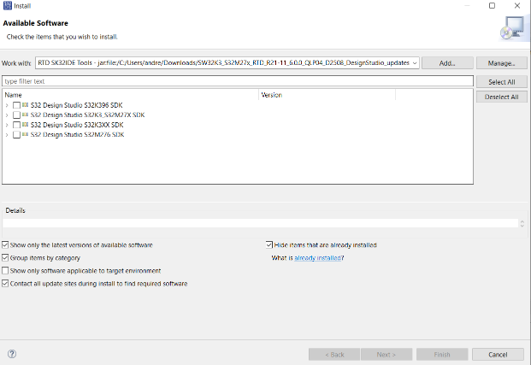
\includegraphics[width=0.8\textwidth]{images/Installation.png}
\end{center}

\newpage

\subsection{Step 2a: Compile Build using RTD Drivers}
Create a new project in S32DS and select the \textbf{S32K3518 board} as your target device.  
Include the \textbf{FreeRTOS kernel} inside the sources and setup the project build config


\begin{center}
    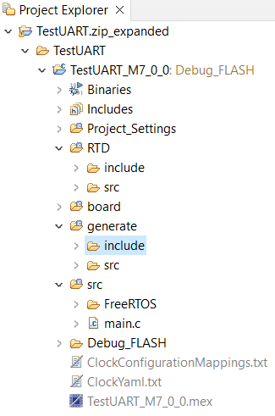
\includegraphics[width=0.5\textwidth]{images/Project_folder.png}
\end{center}
\newpage

\subsection{Step 2b: Adding Drivers Using a MEX File}
S32DS uses \textbf{.mex configuration files} to configure and maintain external peripherals driver settings.
Opening the .mex file allows for editing parameters for the UART, ADC, and other RTD components.

Once the configuration is complete, build the project

\vspace{0.5cm}
\begin{center}
    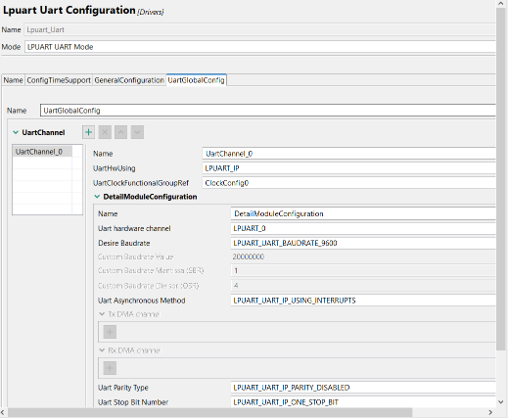
\includegraphics[width=0.8\textwidth]{images/Uart_config.png}
\end{center}


\subsection{Step 2c: Building the Project}
With everything configured, you are ready to build the project.  
Use the compiler provided with S32DS and include the \texttt{-g3} flag to enable detailed debugging information.

An executable file in\textbf{ELF format} (\texttt{.elf}) will be created, and it can be set as the default kernel image for the 

\vspace{0.5cm}
\begin{center}
    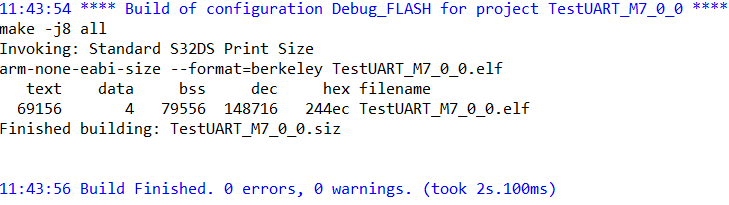
\includegraphics[width=0.75\textwidth]{images/build_output.png}
\end{center}

\subsection{Step 3: Running the Project in QEMU}
After compilation, running
\begin{minted}[fontsize=\small, bgcolor=gray!10, frame=single]{bash}
make qemu_start_temp
\end{minted}


launches our custom QEMU emulation, loads the compiled ELF file, loads the startup.s file and jumps to the first Interrupt vector entry.
Gdb debugging allows for side-stepping the instructions.

\vspace{0.5cm}
\begin{center}
    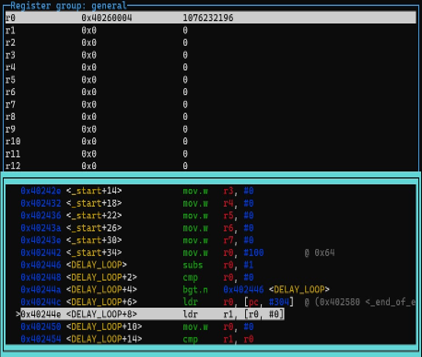
\includegraphics[width=0.5\textwidth]{images/Layout_regs.png}
\end{center}
\vspace{0.5cm}
\begin{center}
    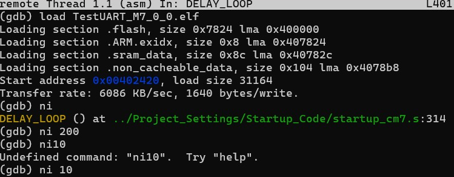
\includegraphics[width=0.5\textwidth]{images/gdb_debug.png}
\end{center}
\vspace{0.5cm}
\begin{center}
    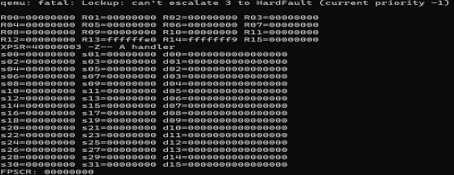
\includegraphics[width=0.5\textwidth]{images/Hard_fault.jpg}
\end{center}


\section{Future Works}
\begin{itemize}
    \item Implementing both the LPUART0 and LPUART1 Low-Power channels
    \item Adding our custom TPM module (Project developed for Cybersecurity for Embedded Systems) to allow secure boot capabilities, RSA key storage and generation, memory access protection from untrusted sources. 
\end{itemize}

\textbf{\href{https://github.com/andreunifi/TPM-Qemu}{Trusted Platform Module repo}}


% ---------------------------
% Bibliography Section
% ---------------------------
\bibliographystyle{plain}    % or IEEEtran, alpha, etc.
\bibliography{references}    % file name of your .bib file (no extension)

\end{document}